\documentclass[useAMS,usenatbib,referee]{biom}
%\documentclass[useAMS,usenatbib,referee]{biom}
%
%
%  Papers submitted to Biometrics should ALWAYS be prepared
%  using the referee option!!!!
%
%
% If your system does not have the AMS fonts version 2.0 installed, then
% remove the useAMS option.
%
% useAMS allows you to obtain upright Greek characters.
% e.g. \umu, \upi etc.  See the section on "Upright Greek characters" in
% this guide for further information.
%
% If you are using AMS 2.0 fonts, bold math letters/symbols are available
% at a larger range of sizes for NFSS release 1 and 2 (using \boldmath or
% preferably \bmath).
%
% The usenatbib command allows the use of Patrick Daly's natbib package for
% cross-referencing.
%
% If you wish to typeset the paper in Times font (if you do not have the
% PostScript Type 1 Computer Modern fonts you will need to do this to get
% smoother fonts in a PDF file) then uncomment the next line
% \usepackage{Times}
%%%%% AUTHORS - PLACE YOUR OWN MACROS HERE %%%%%

\usepackage[figuresright]{rotating}
\usepackage{tikz}
\usepackage{amsmath}
\usepackage[hyphens]{url} % not crucial - just used below for the URL
\usepackage{hyperref}
\usepackage[utf8]{inputenc}
\usepackage{graphicx}
\usepackage{longtable}
\usepackage{booktabs}
%% \raggedbottom % To avoid glue in typesetteing, sbs>>

% Pandoc syntax highlighting
\usepackage{color}
\usepackage{fancyvrb}
\newcommand{\VerbBar}{|}
\newcommand{\VERB}{\Verb[commandchars=\\\{\}]}
\DefineVerbatimEnvironment{Highlighting}{Verbatim}{commandchars=\\\{\}}
% Add ',fontsize=\small' for more characters per line
\usepackage{framed}
\definecolor{shadecolor}{RGB}{248,248,248}
\newenvironment{Shaded}{\begin{snugshade}}{\end{snugshade}}
\newcommand{\AlertTok}[1]{\textcolor[rgb]{0.94,0.16,0.16}{#1}}
\newcommand{\AnnotationTok}[1]{\textcolor[rgb]{0.56,0.35,0.01}{\textbf{\textit{#1}}}}
\newcommand{\AttributeTok}[1]{\textcolor[rgb]{0.77,0.63,0.00}{#1}}
\newcommand{\BaseNTok}[1]{\textcolor[rgb]{0.00,0.00,0.81}{#1}}
\newcommand{\BuiltInTok}[1]{#1}
\newcommand{\CharTok}[1]{\textcolor[rgb]{0.31,0.60,0.02}{#1}}
\newcommand{\CommentTok}[1]{\textcolor[rgb]{0.56,0.35,0.01}{\textit{#1}}}
\newcommand{\CommentVarTok}[1]{\textcolor[rgb]{0.56,0.35,0.01}{\textbf{\textit{#1}}}}
\newcommand{\ConstantTok}[1]{\textcolor[rgb]{0.00,0.00,0.00}{#1}}
\newcommand{\ControlFlowTok}[1]{\textcolor[rgb]{0.13,0.29,0.53}{\textbf{#1}}}
\newcommand{\DataTypeTok}[1]{\textcolor[rgb]{0.13,0.29,0.53}{#1}}
\newcommand{\DecValTok}[1]{\textcolor[rgb]{0.00,0.00,0.81}{#1}}
\newcommand{\DocumentationTok}[1]{\textcolor[rgb]{0.56,0.35,0.01}{\textbf{\textit{#1}}}}
\newcommand{\ErrorTok}[1]{\textcolor[rgb]{0.64,0.00,0.00}{\textbf{#1}}}
\newcommand{\ExtensionTok}[1]{#1}
\newcommand{\FloatTok}[1]{\textcolor[rgb]{0.00,0.00,0.81}{#1}}
\newcommand{\FunctionTok}[1]{\textcolor[rgb]{0.00,0.00,0.00}{#1}}
\newcommand{\ImportTok}[1]{#1}
\newcommand{\InformationTok}[1]{\textcolor[rgb]{0.56,0.35,0.01}{\textbf{\textit{#1}}}}
\newcommand{\KeywordTok}[1]{\textcolor[rgb]{0.13,0.29,0.53}{\textbf{#1}}}
\newcommand{\NormalTok}[1]{#1}
\newcommand{\OperatorTok}[1]{\textcolor[rgb]{0.81,0.36,0.00}{\textbf{#1}}}
\newcommand{\OtherTok}[1]{\textcolor[rgb]{0.56,0.35,0.01}{#1}}
\newcommand{\PreprocessorTok}[1]{\textcolor[rgb]{0.56,0.35,0.01}{\textit{#1}}}
\newcommand{\RegionMarkerTok}[1]{#1}
\newcommand{\SpecialCharTok}[1]{\textcolor[rgb]{0.00,0.00,0.00}{#1}}
\newcommand{\SpecialStringTok}[1]{\textcolor[rgb]{0.31,0.60,0.02}{#1}}
\newcommand{\StringTok}[1]{\textcolor[rgb]{0.31,0.60,0.02}{#1}}
\newcommand{\VariableTok}[1]{\textcolor[rgb]{0.00,0.00,0.00}{#1}}
\newcommand{\VerbatimStringTok}[1]{\textcolor[rgb]{0.31,0.60,0.02}{#1}}
\newcommand{\WarningTok}[1]{\textcolor[rgb]{0.56,0.35,0.01}{\textbf{\textit{#1}}}}

% tightlist command for lists without linebreak
\providecommand{\tightlist}{%
  \setlength{\itemsep}{0pt}\setlength{\parskip}{0pt}}



%%%%%%%%%%%%%%%%%%%%%%%%%%%%%%%%%%%%%%%%%%%%%%%%

\setcounter{footnote}{2}

\title[]{Title here}

\author{ Author
1 \email{\href{mailto:abc@def}{\nolinkurl{abc@def}}} \\ Department of
YYY, University of XXX  \and
		 Author
2 \email{\href{mailto:djf@wef}{\nolinkurl{djf@wef}}} \\ Department of
ZZZ, University of WWW 
	   }


\begin{document}


\date{{\it Received May} 2022}

\pagerange{\pageref{firstpage}--\pageref{lastpage}} \pubyear{2022}

\volume{0}
\artmonth{January}
\doi{0000-0000-0000}

%  This label and the label ``lastpage'' are used by the \pagerange
%  command above to give the page range for the article

\label{firstpage}

%  pub the summary here

\begin{abstract}
The text of your summary. Should not exceed 225 words.
\end{abstract}

%
%  Please place your key words in alphabetical order, separated
%  by semicolons, with the first letter of the first word capitalized,
%  and a period at the end of the list.
%

\begin{keywords}
keydictionaryword.
\end{keywords}

\maketitle

\hypertarget{intro}{%
\section{Introduction}\label{intro}}

Your text comes here. Separate text sections with

\hypertarget{sec:1}{%
\section{Section title}\label{sec:1}}

Text with citations by \citet{heagerty2000time},
\citep{pepe2003statistical}.

\hypertarget{sec:2}{%
\subsection{Subsection title}\label{sec:2}}

as required \citep{hoerl1970ridge, zou2005regularization}. Don't forget
to give each section and subsection a unique label (see Sect.
\ref{sec:1}).

\hypertarget{paragraph-headings}{%
\paragraph{Paragraph headings}\label{paragraph-headings}}

Use paragraph headings as needed.

\hypertarget{equations}{%
\subsection{Equations}\label{equations}}

Here is an equation:

\[ f_{X}(x) = \left(\frac{\alpha}{\beta}\right)\left(\frac{x}{\beta}\right)^{\alpha-1}e^{-\left(\frac{x}{\beta}\right)^{\alpha}}; \alpha,\beta,x > 0 \]

Here is another: \begin{align}
a^2+b^2=c^2
\end{align}

Inline equations: \(\sum_{i = 2}^\infty\{\alpha_i^\beta\}\)

\hypertarget{figures-and-tables}{%
\section{Figures and tables}\label{figures-and-tables}}

\hypertarget{figures-coming-from-r}{%
\subsection{Figures coming from R}\label{figures-coming-from-r}}

\hypertarget{normal-figure-embedded-in-text}{%
\paragraph{Normal figure embedded in
text}\label{normal-figure-embedded-in-text}}

\begin{verbatim}
## Warning in plot.formula(runif(25) ~ runif(25)): the formula 'runif(25) ~
## runif(25)' is treated as 'runif(25) ~ 1'
\end{verbatim}

\begin{figure}
\centering
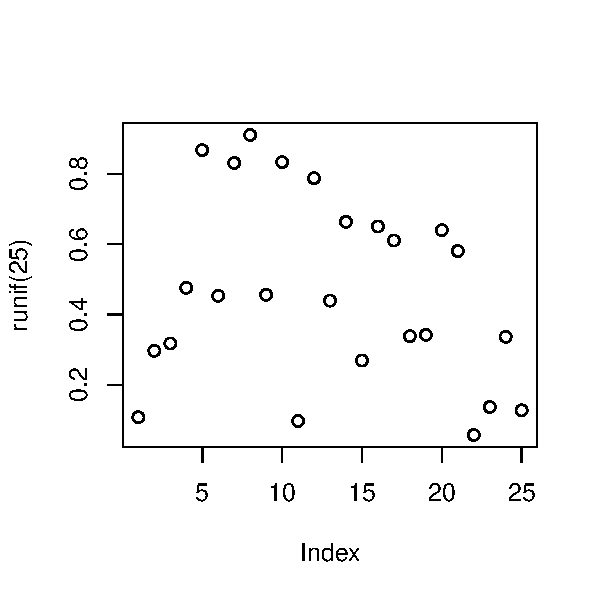
\includegraphics{BJAII_files/figure-latex/fig2-1.pdf}
\caption{Output from \texttt{pdf()}}
\end{figure}

\clearpage

\hypertarget{tables-coming-from-r}{%
\subsection{Tables coming from R}\label{tables-coming-from-r}}

\begin{Shaded}
\begin{Highlighting}[]
\FunctionTok{print}\NormalTok{(xtable}\SpecialCharTok{::}\FunctionTok{xtable}\NormalTok{(}\FunctionTok{head}\NormalTok{(mtcars)[,}\DecValTok{1}\SpecialCharTok{:}\DecValTok{4}\NormalTok{], }
\AttributeTok{caption =} \StringTok{"Caption centered under table"}\NormalTok{, }\AttributeTok{label =} \StringTok{"tab1"}\NormalTok{), }
\AttributeTok{comment =} \ConstantTok{FALSE}\NormalTok{, }\AttributeTok{timestamp =} \ConstantTok{FALSE}\NormalTok{, }\AttributeTok{caption.placement =} \StringTok{"top"}\NormalTok{)}
\end{Highlighting}
\end{Shaded}

\begin{table}[ht]
\centering
\caption{Caption centered under table} 
\label{tab1}
\begin{tabular}{rrrrr}
  \hline
 & mpg & cyl & disp & hp \\ 
  \hline
Mazda RX4 & 21.00 & 6.00 & 160.00 & 110.00 \\ 
  Mazda RX4 Wag & 21.00 & 6.00 & 160.00 & 110.00 \\ 
  Datsun 710 & 22.80 & 4.00 & 108.00 & 93.00 \\ 
  Hornet 4 Drive & 21.40 & 6.00 & 258.00 & 110.00 \\ 
  Hornet Sportabout & 18.70 & 8.00 & 360.00 & 175.00 \\ 
  Valiant & 18.10 & 6.00 & 225.00 & 105.00 \\ 
   \hline
\end{tabular}
\end{table}

Table \ref{tab1} shows these numbers. Some of those numbers are plotted
in Figure \ref{fig:fig1}.

\begin{Shaded}
\begin{Highlighting}[]
\FunctionTok{head}\NormalTok{(mtcars[,}\DecValTok{1}\SpecialCharTok{:}\DecValTok{4}\NormalTok{])}
\end{Highlighting}
\end{Shaded}

\begin{verbatim}
##                    mpg cyl disp  hp
## Mazda RX4         21.0   6  160 110
## Mazda RX4 Wag     21.0   6  160 110
## Datsun 710        22.8   4  108  93
## Hornet 4 Drive    21.4   6  258 110
## Hornet Sportabout 18.7   8  360 175
## Valiant           18.1   6  225 105
\end{verbatim}


\bibliographystyle{biom}
\bibliography{bibliography.bib}


\label{lastpage}


\end{document}
